\documentclass[notes]{beamer}
\usepackage{hyperref}
\usepackage[T1]{fontenc}
\UseRawInputEncoding

\usepackage{pgfpages}
\setbeameroption{show notes on second screen=right}
%\usepackage[backend=biber]{biblatex} 
\usepackage[square,comma,numbers]{natbib}

% other packages
\usepackage{latexsym,amsmath,xcolor,multicol,booktabs,calligra}
\usepackage{graphicx,listings,stackengine,subfig}
\usepackage{multirow}
\renewcommand{\footnotesize}{\tiny}

\title{Multiclass Classification Of Leptons In Proton-Proton Collisions At \textsurd s=13 TeV Using Machine Learning}
\author{Kristoffer Langstad}
\institute{University of Oslo, Department of Physics}
\date{\today}


\begin{document}
	\begin{frame}[t]{Thesis Presentation}
		\titlepage
	\end{frame}


	\begin{frame}[t]{Outline}
		\begin{enumerate}
			\item Introduction
				\begin{enumerate}[(i)]
					\item Particle physics model
					\item Central Machine Learning concepts
				\end{enumerate}
			\item Multiclass Classification
			\item Results
			\item Summary, Conclusion, Outlook
		\end{enumerate}
	\end{frame}
	\note{
		\begin{enumerate}
			\item Introduction
			\begin{enumerate}[(i)]
				\item Particle physics model
				\item Central Machine Learning concepts
			\end{enumerate}
			\item Multiclass Classification
			\item Results
			\item Summary, Conclusion, Outlook
		\end{enumerate}
	}


	\begin{frame}[t]{Standard Model}
		\begin{figure}[ht!]
			\centering
			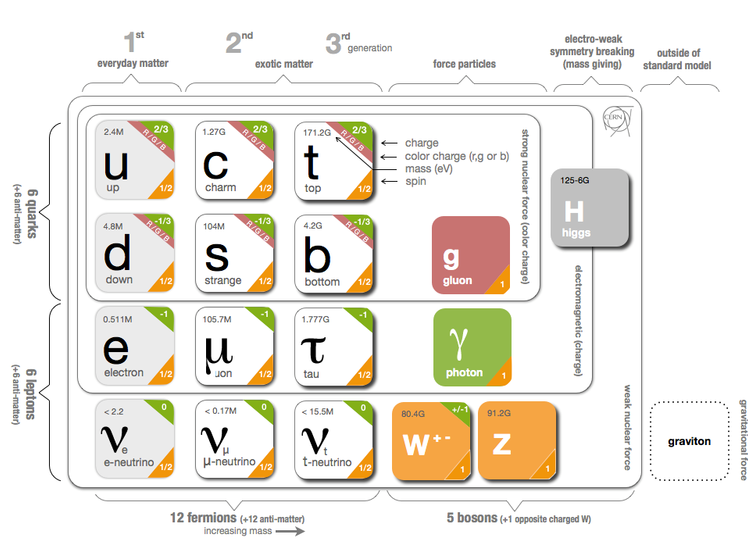
\includegraphics[width=0.8\linewidth]{SM.png}
			\caption{The Standard Model contents, source \cite{SM}. \label{fig:SM}}
		\end{figure} 
	\end{frame}
	\note{
		SM explain with great precision. Fundamental particles in figure w/ charge, spin and mass.
		Does not explain graviton and non-zero mass of neutrino.
		
		Introduce Inverse seesaw mechanism w/ heavy neutrinos and right-handed neutrinos. Left-handed for all SM particles, and LH means direction of spin and motion are opposite. ISS-> trilepton final state with a neutrino through p-p collisions and decay through W-boson and heavy pseudo-Dirac neutrino.
	}


	\begin{frame}[t]{Trilepton Final State}
		\begin{figure}[htbp!]
			\centering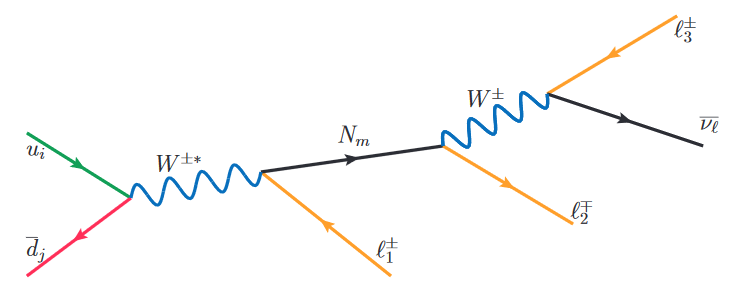
\includegraphics[width=0.8\linewidth]{ModelProcess.png}
			\caption{The Born diagram for the charged current Drell-Yan process of the proton-proton collision (on the left) producing a heavy pseudo-Dirac neutrino $N$ in the inverse seesaw mechanism model, leading to a trilepton plus missing transverse energy (a light neutrino) final state. Figure is taken from ref. \citet{inverseseesaw}. \label{fig:ModelProcessIntro}}
		\end{figure}
	\end{frame}
	\note{
		Figure of P-P collisions to trilepton final state and decays. Charges. At LHC and CERN, detected by ATLAS but neutrinos are not. Only MET since conservation of energy.
		
		Called charged current Drell-Yan process, same model we look at for neutrinos as by \citet{inverseseesaw}. Gives almost conserved lepton number and consider only electrons and muons. Amount of SS and OS events vertex 1 and 2 differ from normal seesaw. Allows LFV for vertex 1 and 2 for e and mu. Study two simulated neutrino signals, mass 150 GeV and 450 GeV, expect different LFV for different neutrino mass models.
		
		Not always trivial to identify particles. P-P collisions simulated, and measure properties like momentum, transverse momentum and coord-angles. Make new variables dPhi, dR and mll.
	}


	\begin{frame}[t]{Machine Learning Process}
		\begin{block}{What we want to do:}
			Use machine learning to identify lepton vertices in simulated backgrounds and signals.
		\end{block}
		\begin{block}{How to do it:}
			\begin{enumerate}[I]
				\item Use supervised learning and multiclass classification.
				\item Train and optimize machine learning algorithms
				\item Evaluate which model that best predicts the vertices.
				\item Predict leptons for simulated backgrounds and signals.
			\end{enumerate}
		\end{block}
		\begin{block}{End goal:}
			\begin{enumerate}[I]
				\item Look for lepton flavor violation between the classified leptons 1 and 2.
				\item Compare with a more standard analysis by \citet{inverseseesaw}.
			\end{enumerate}
		\end{block}
	\end{frame}
	\note{
		Machine learning to train to identify the particles vertices, pattern recognition in particle properties. Truth simulated data, know the origins and what particles have been produced. Train various ML algorithms, use best performing model to predict simulated backgrounds and signals. Six different lepton vertex permutations. Multiclass classification case with six classes, not been studied much previously in particle physics. 
		
		Need good and fast algorithms for classification, lot of data to work with. Need preprocessing of data before classification. Train models on training set. Many hyperparameters to optimize on validation set. Evaluation metrics for performance evaluation for validation and test set. Export best model, skips training the models each time.
		
		Signal region cuts to study LFV for lepton 1 and 2. Compare with a more standard analysis by Pascoli et al.
	}


	\begin{frame}[t]{Preprocessing of Data}
		\begin{enumerate}[(i)]
			\item Feature correlations
			\item Resampling
			\item Splitting into data sets
			\item Scaling
		\end{enumerate}
	\end{frame}
	\note{
		...
	}


	\begin{frame}[t]{Bias-Variance Tradeoff}
		\begin{figure}[htbp!]
			\centering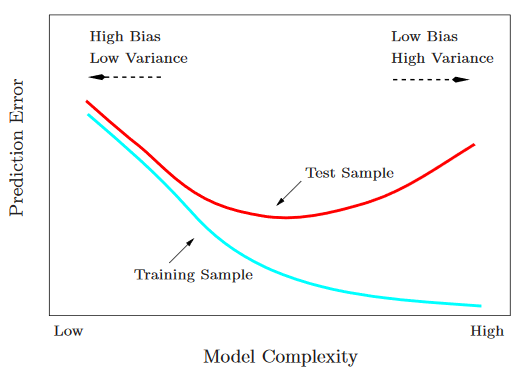
\includegraphics[width=0.8\linewidth]{bias-variance.png}
			\caption{Illustration of the quality of a model from how well it does on data not seen during training with variance and bias regions. Source by \citet{mehta2019high}. \label{fig:BiasVar}}
		\end{figure}
	\end{frame}
	\note{
		...
	}


	\begin{frame}[t]{Classification Algorithms}
		Types of classification algorithms used:
		\begin{enumerate}[(i)]
			\item Logistic regression
			\item Multi-layer perceptron
			\item Trees
			\item Boosters
			\item Multiclassifiers
		\end{enumerate}
	\end{frame}
	\note{
		...
	}


	\begin{frame}[t]{Classification Results}
		\begin{table}[htbp!]
			\centering
			%\hspace{-1cm}
			\begin{tabular}{ |c|c|c|c|c| }
				\hline \rule{0pt}{13pt}
				\multirow{2}{*}{Model} & \multicolumn{4}{c|}{Signal models} \\
				\cline{2-5} \rule{0pt}{13pt}
				 & \multicolumn{2}{c|}{150 GeV} & \multicolumn{2}{c|}{450 GeV} \\
				\cline{2-5} \rule{0pt}{13pt}
				 & Score & Score\_train & Score & Score\_train \\
				\hline \rule{0pt}{13pt}
				AdaBoost & 0.8519 & 1.0000 & 0.9385 & 1.0000 \\
				\hline \rule{0pt}{13pt}
				OvO & 0.7788 & 0.9299 & 0.9088 & 0.9319 \\
				\hline \rule{0pt}{13pt}
				MLP & 0.8227 & 0.9492 & 0.9350 & 0.9606 \\
				\hline \rule{0pt}{13pt}
				HGBC & 0.7863 & 0.8999 & 0.9280 & 0.9571 \\
				\hline \rule{0pt}{13pt}
				XGBoost & 0.8631 & 0.9998 & 0.9509 & 0.9999 \\
				\hline \rule{0pt}{13pt}
				LGBM & \textbf{0.8779} & 0.9999 & \textbf{0.9541} & 0.9999\\
				\hline
			\end{tabular}	
			\caption{Table containing accuracy scores of the highest performing classification models trained on the 150 GeV and 450 GeV validation and training sets.}
			\label{tab:Validation}
		\end{table}
	\end{frame}
	\note{
		...
	}


	\begin{frame}[t]{Light Gradient Boosting Machine}
		\begin{figure}[h]
			\centering
			\subfloat{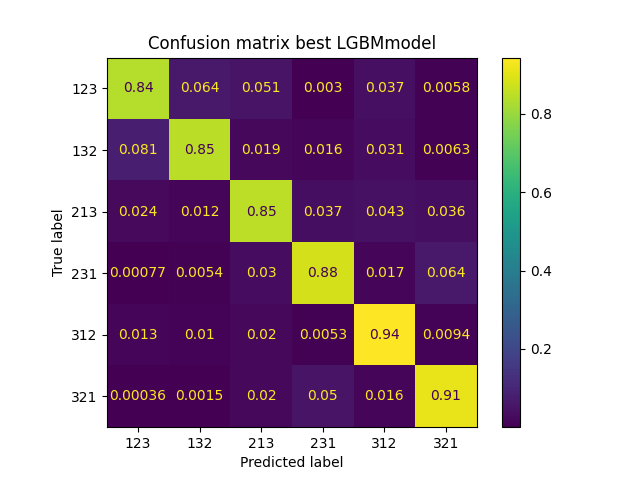
\includegraphics[width=0.5\textwidth]{Test_plots/Conf_mat_150.png}}
			\subfloat{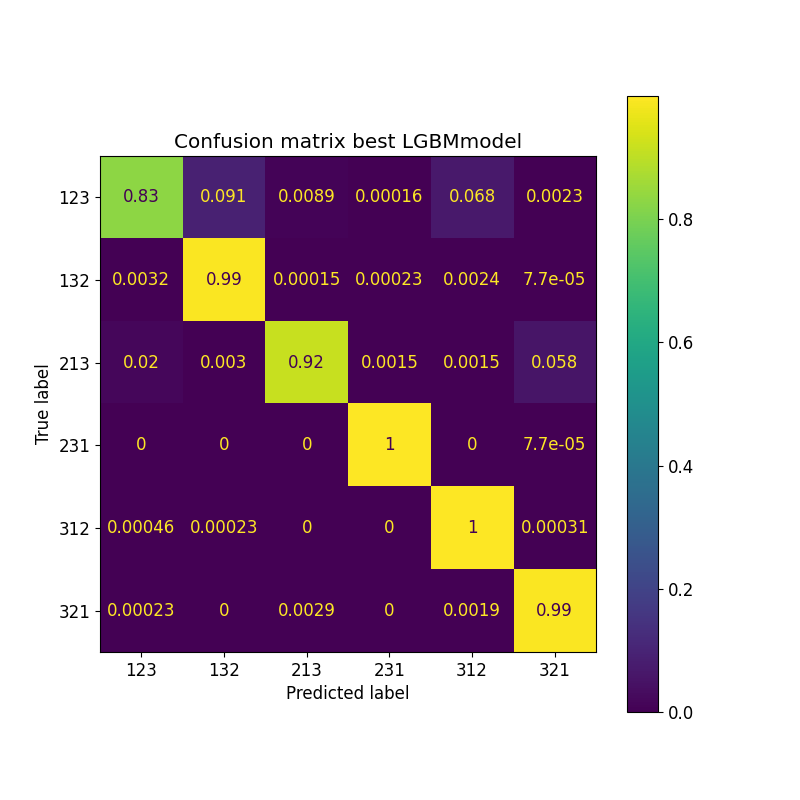
\includegraphics[width=0.5\textwidth]{Test_plots/Conf_mat_450.png}}
			\caption{Light Gradient Boosting Mechanism confusion matrix on the test set for both signals.}
		\end{figure}
	\end{frame}
	\note{
		...
	}


	\begin{frame}[t]{Scores}
		\begin{table}[htb!]
			%\hspace{-0.8cm}
			\centering
			\begin{tabular}{ |c|c|c|c|c| }
				\hline \rule{0pt}{13pt}
				Signal [GeV] & Score & Score\_train & CKS & LogLoss  \\
				\hline \rule{0pt}{13pt}
				150 & 0.8793 & 0.9999 & 0.8551 & 0.3335 \\
				\hline \rule{0pt}{13pt}
				450 & 0.9570 & 0.9999 & 0.9484 & 0.1120 \\
				\hline
			\end{tabular}	         
			\caption{Accuracy score of both the test and training sets, Cohen Kappe score and logloss for both the 150 and 450 GeV signal models.}
			\label{tab:Test}
		\end{table}
		\begin{table}[htb!]
			%\hspace{-0.8cm}
			\centering
			\begin{tabular}{ |c|c|c|c| }
				\hline \rule{0pt}{13pt}
				\multirow{2}{*}{Signal [GeV]} & \multicolumn{2}{c|}{ROC} & \multicolumn{1}{c|}{Precision-Recall}\\
				\cline{2-4} \rule{0pt}{13pt}
				 & Micro AUC & Macro AUC & Micro AUC  \\
				\hline \rule{0pt}{13pt}
				150 & 0.99 & 0.99 & 0.949 \\
				\hline \rule{0pt}{13pt}
				450 & 1.0 & 1.0 & 0.994  \\
				\hline
			\end{tabular}	         
			\caption{Area under the curve (AUC) scores for both ROC and precision-recall curves..}
			\label{tab:AUC}
		\end{table}
	\end{frame}
	\note{
		...
	}



%--------------
	\begin{frame}[t]{References}
		\bibliographystyle{unsrtnat} %plain, unsrt, abbrv
		\bibliography{Refs}
	\end{frame}

\end{document}
